\section{Beam line detectors}
\subsection{Overview}
\begin{figure}[htbp]
  \centering
  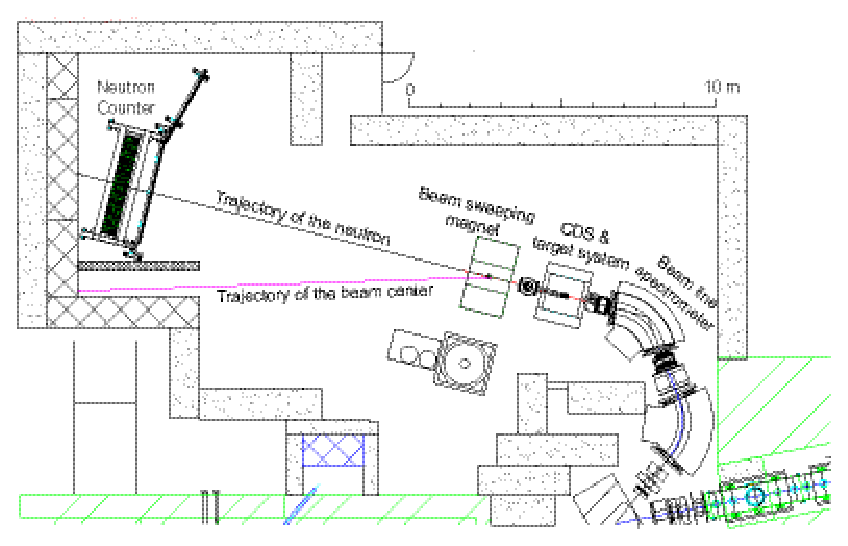
\includegraphics[width=8cm]{pic/experiment/hall.eps}
  \caption{
    Schematic view of the experimental hall at the K1.8BR.
  }
\end{figure}

\begin{figure}[htbp]
  \begin{tabular}{cc}
    \begin{minipage}{0.4\hsize}
      \begin{centering}
        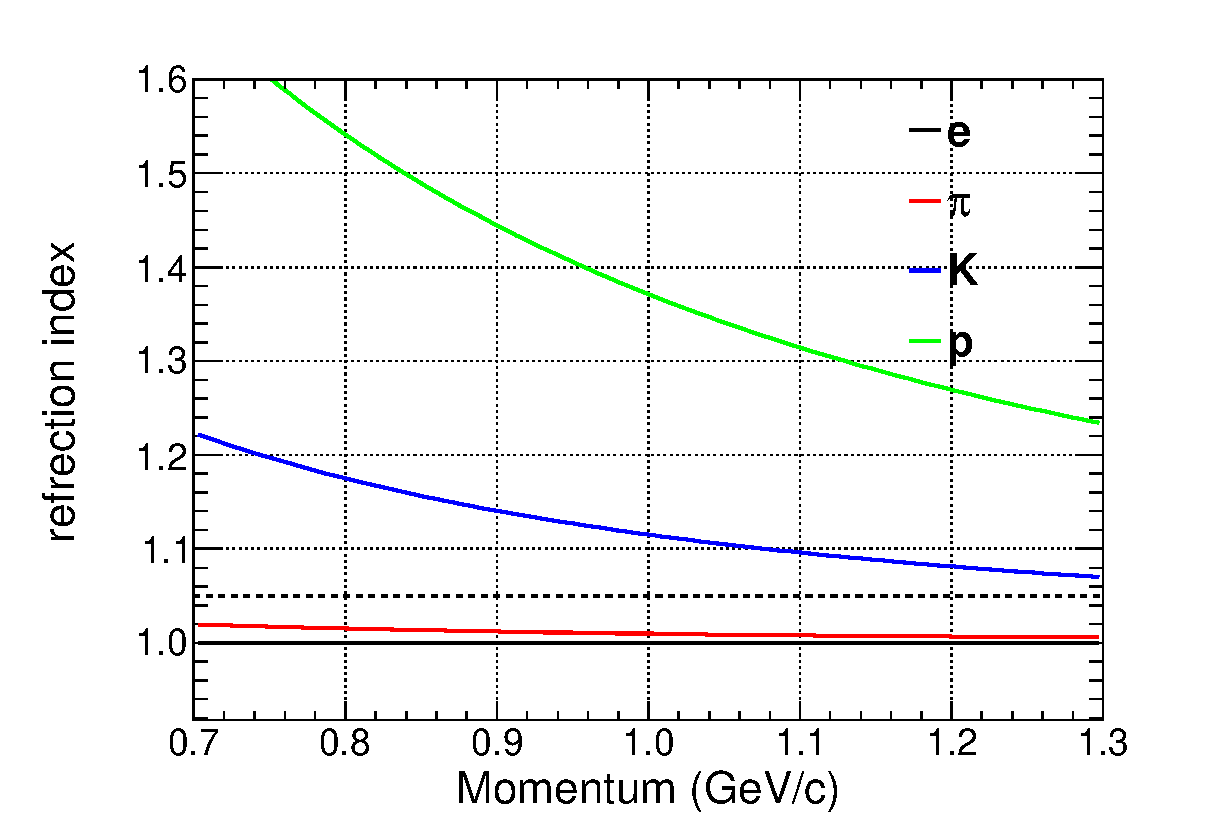
\includegraphics[width=5cm]{pic/experiment/ACthre.eps}
      \end{centering}
    \end{minipage}
    \begin{minipage}{0.6\hsize}
      \begin{centering}
        \includegraphics[width=7cm]{pic/experiment/newac.eps}
      \end{centering}
    \end{minipage}
  \end{tabular}
  \caption{
    The right figure shows a schematic drawing of the AC.
    The left figure represents the threshold of reflection index for Cherenkov radiation and the momentum. The horizontal dotted line shows the reflection index of the Aerogel (n=1.05).
  }
  \label{fig:AC}
\end{figure}
A kaon was identified by threshold type of aerogel Cherenkov counter (AC) with refractive index $n=1.05$ which can identify kaon and pion around $0.7\sim1.2 GeV/c$ as Fig\ref{fig:AC}.
This offline level identification information was used for beam line tuning, especially koan and another particle separation.
We first search ES1 voltage and CM1/2 current which maximize kaon yield.
After that, IF slit and MS1 slit were adjusted to maximize the number of kaons while keeping an acceptable level of pion contamination.
In this tuning, vertical direction opening width was decided to avoid pion peak come from direct production at the T1 target and
horizontal direction was set to reject pion come from magnets and so on installed in beamline which so-call pion hallo.

The beam particle identification was also performed using the TOF method by beamline hodoscope counter (BHD) and time-zero (T0) counter which has about $7.7m$ flight length.
The T0 counter was installed at downstream of D5 magnet and was rotated by 45 degrees about the beam direction axis,
which consists of 5 segmented plastic scintillation counters whose size is 160mm (height) $\times$ 32mm (width) $\times$ 10mm (thickness),
so the T0 counter covers 160mm $\times$ 160mm effective area.
A counter uses the Saint-Gobain BC420 scintillator and attached readout which is 3/4 inch Hamamatsu H6612B photomultipliers to both sides of the scintillator.

The BHD counter was installed at just upstream of the D4 magnet,
which consists of 20 segment plastic scintillaton counters whose size is 160mm (height) $\times$ 20mm (width) $\times$ 5mm (thickness),
so the BHD counter covers 400mm (horizontal) $\times$ 160mm (vertical) effective area.
A counter uses the same photomultipliers as the T0 counter.
Since beam rate was a few M events per spill, photomultipliers were attached high voltage booster to the last three dynodes to avoid gain drop due to high current by high rate beam.
